\documentclass[conference]{IEEEtran}
\IEEEoverridecommandlockouts

\usepackage{cite}
\usepackage{amsmath,amssymb,amsfonts}
\usepackage{algorithmic}
\usepackage{algorithm}
\usepackage{graphicx}
\usepackage{textcomp}
\usepackage{xcolor}
\usepackage{booktabs}
\usepackage{array}
\usepackage{multirow}
\usepackage{url}
\usepackage{pifont}
\usepackage{hyperref}
\usepackage{amsthm}
\usepackage{tikz}
\usetikzlibrary{shapes.geometric,arrows.meta,positioning,calc}
\usepackage{pgfplots}
\pgfplotsset{compat=1.18}
\usepgfplotslibrary{statistics}
\newtheorem{definition}{Definition}

\def\BibTeX{{\rm B\kern-.05em{\sc i\kern-.025em b}\kern-.08em
    T\kern-.1667em\lower.7ex\hbox{E}\kern-.125emX}}

\newcommand{\cmark}{\ding{51}}
\newcommand{\xmark}{\ding{55}}
\newcommand{\pmark}{\textasciitilde}

\begin{document}

\title{CapAI: A Self-Expanding, Sandbox-Verified Capability Acquisition
       Layer for Large and Small Language Models}

\author{
  \IEEEauthorblockN{Sanjay Varma, Harshitha P, Gandhar, Revathi GP}
  \IEEEauthorblockA{PES University, Bengaluru, India}
}

\maketitle

%-----------------------------------------------------------------------
\begin{abstract}
Large language models (LLMs) incur repeated latency and inference cost
because every invocation is stateless and correctness is never verified.
This problem is especially severe for small, locally-deployable models
that frequently produce fluent but logically incorrect output.
We propose \textbf{CapAI}, a self-expanding capability acquisition layer
that converts natural-language requests into sandbox-verified, permanently
cached software artifacts synthesized once and retrieved instantly by any
subsequent caller. CapAI combines a tiered synthesis architecture---a
deterministic heuristic library, single-function LLM synthesis, and a
five-stage class and pipeline synthesis architecture with coverage-guided
iterative repair---a MongoDB-backed persistent capability registry, a
Python client interface, and a Model Context Protocol~(MCP) server
exposing capabilities as native tools.
Cached retrieval achieves a measured mean latency of 1{,}095.3~ms versus
6{,}730.6~ms for first-time synthesis, a 6.14$\times$ reduction confirmed
at $p < 10^{-6}$ (Welch's $t = 42.87$, Cohen's $d = 1.97$,
$n = 3{,}080$ trials across 150~capability types).
An advanced-build benchmark records an 85.9\% success rate across
92~independent trials on 29~capability types.
A four-condition ablation study confirms that the repair loop contributes
27.4~percentage points of build success, and that persistence prevents a
46.7~percentage point correctness collapse across server restarts.
A multi-model evaluation across 8B, 20B, and 70B parameter models shows
equivalent Pass@1 (86.7\%), indicating model-size independence for the
capability types evaluated.
On HumanEval, CapAI achieves 34.9\% Pass@1 across 149~tasks.
Critically, no incorrect outputs were observed among the 40~evaluated
uncached baseline executions, whereas the cached path achieved 83.0\%
correctness, because a single verification miss, once persisted,
propagates silently to every subsequent retrieval.
These findings indicate that verification quality, rather than persistence
alone, is a key determinant of whether capability caching improves overall
system reliability.
\end{abstract}

\begin{IEEEkeywords}
large language models, code generation, tool use, Model Context Protocol,
self-healing code, sandboxed execution, capability caching, semantic
similarity matching, statistical evaluation
\end{IEEEkeywords}

%=======================================================================
\section{Introduction}
\label{sec:introduction}
%=======================================================================

Large language models (LLMs) have evolved from text-completion engines
into general-purpose computational assistants capable of writing,
executing, and reasoning about code.
Modern LLM-serving infrastructure---exemplified by Groq, Cerebras, and
NVIDIA NIM---has made it inexpensive and fast to request synthesised code
on demand, while the Model Context Protocol
(MCP)~\cite{anthropic_mcp2024} has emerged as a uniform interface for
exposing AI-accessible tools.
Despite this abundance of fast, low-cost inference, a structural
inefficiency persists: LLM calls are stateless.
An agent that requests \texttt{is\_prime(n)} today pays the full
synthesis cost again tomorrow, with no mechanism to recognise that the two
requests address the same underlying capability.
Furthermore, correctness is assumed rather than verified, a risk that is
especially acute for small models (under 4B parameters) that frequently
hallucinate arithmetic and off-by-one logic.

\subsection{What Is CapAI?}

CapAI is a \emph{self-expanding capability acquisition layer}.
It treats every successfully synthesised and sandbox-verified function,
class, or pipeline as a permanent, reusable software artifact rather than
a disposable generation.
When a requested capability is absent from CapAI's persistent capability
registry, it is synthesised by an LLM, executed inside an isolated
sandbox, and---only if it passes verification---promoted to MongoDB-backed
storage.
Every subsequent request for that capability, from any caller, retrieves
the verified artifact directly, bypassing LLM inference entirely.

\subsection{Why Existing Systems Are Insufficient}
\label{subsec:why_existing}

Several systems address adjacent problems, yet none combines verified
persistence with native tool-protocol exposure:

\begin{itemize}
  \item \textbf{GPTCache}~\cite{gptcache2023} caches responses by
        embedding similarity but applies no correctness verification---a
        cache hit is defined by similarity, not by execution.
  \item \textbf{Reflexion}~\cite{shinn2023reflexion} repairs responses via
        verbal reinforcement but does not persist verified artifacts
        across sessions.
  \item \textbf{Voyager}~\cite{wang2023voyager} stores agent skills for a
        game environment; skills are environment-specific and not exposed
        as reusable software assets or MCP tools.
  \item \textbf{OpenHands}~\cite{wang2024openhands} provides sandboxed
        code execution but does not cache verified results for reuse by
        independent callers.
  \item \textbf{SWE-Agent}~\cite{yang2024sweagent} and
        \textbf{MetaGPT}~\cite{hong2023metagpt} orchestrate multi-agent
        software engineering but do not persist executable artifacts for
        zero-latency retrieval.
  \item \textbf{DSPy}~\cite{khattab2023dspy} compiles prompt pipelines;
        it addresses prompt efficiency, not verified capability persistence.
\end{itemize}

CapAI uniquely stores \textbf{verified executable capabilities} that
become reusable software assets and exposes them as native MCP tools to
any compatible agent.

\subsection{Contributions}

This paper makes the following contributions:
\begin{enumerate}
  \item A complete tiered synthesis architecture combining a verified
        heuristic library, single-function LLM synthesis, and a five-stage
        class and pipeline synthesis architecture with coverage-guided
        iterative self-repair.
  \item A persistent capability registry yielding a measured 6.14$\times$
        latency reduction, confirmed at $p < 10^{-6}$ across 150~capability
        types and 3{,}080~trials.
  \item A controlled, repeated-trial experimental evaluation at scale
        (190~tasks, 3{,}337~trials) with statistical significance testing,
        effect sizes, and Wilson score confidence intervals, including a
        genuine negative result; and a four-condition ablation study
        isolating the contribution of caching, the repair loop, MCP
        exposure, and persistence.
  \item Empirical support for the hand-designed confidence score formula,
        with Pearson $r = 0.79$ between confidence scores and
        ground-truth correctness.
  \item A multi-model evaluation demonstrating that CapAI's verification
        and repair pipeline achieves equivalent Pass@1 (86.7\%) across
        models of substantially different sizes (8B, 20B, and 70B
        parameters), indicating model-size independence for the capability
        types evaluated.
  \item A HumanEval evaluation reporting 34.9\% Pass@1 across 149~tasks,
        enabling direct comparison with published code generation systems.
  \item Native exposure of the system as an MCP server.
  \item An empirical case study integrating CapAI with a small,
        locally-hosted language model.
  \item Five prototype extensions toward a fuller research agenda.
\end{enumerate}

\subsection{Paper Organization}

The remainder of this paper is organized as follows.
Section~\ref{sec:problem} defines the research problem and hypotheses.
Section~\ref{sec:formal} provides a formal definition of a capability.
Section~\ref{sec:related} reviews related work.
Section~\ref{sec:architecture} describes the system architecture.
Section~\ref{sec:methods} presents the synthesis and retrieval algorithms.
Section~\ref{sec:complexity} analyzes computational complexity.
Section~\ref{sec:evaluation} reports experimental results.
Section~\ref{sec:ablation} presents the ablation study.
Sections~\ref{sec:casestudy} and~\ref{sec:extensions} present the local
model case study and prototype extensions.
Sections~\ref{sec:security}--\ref{sec:reproducibility} address security,
ethics, discussion, and reproducibility.
Section~\ref{sec:conclusion} concludes.

%=======================================================================
\section{Problem Statement and Research Questions}
\label{sec:problem}
%=======================================================================

\subsection{Research Problem}

\textit{Can verified capability persistence reduce repeated inference cost
while maintaining correctness, and under what conditions does persistence
improve or degrade aggregate system reliability?}

\subsection{Research Questions}

\begin{description}
  \item[RQ1] Does capability caching reduce latency relative to direct LLM
        inference?
  \item[RQ2] Under what conditions does sandboxed verification influence
        the correctness of persisted capabilities?
  \item[RQ3] Does capability persistence outperform repeated stateless
        generation in aggregate correctness across repeated invocations?
\end{description}

\subsection{Hypothesis}

\textit{Verified reusable capabilities outperform stateless generation
under repeated workloads when verification quality is sufficiently high;
however, a verification blind spot, once persisted, degrades aggregate
correctness more severely than independent regeneration errors.}

%=======================================================================
\section{Formal Definition}
\label{sec:formal}
%=======================================================================

\begin{definition}[Capability]
A \emph{capability} $\mathcal{C}$ is a 5-tuple
$\langle k, \sigma, \mathcal{F}, \mathcal{T}, \rho \rangle$ where:
\begin{itemize}
  \item $k \in \Sigma^*$ is a stable string identifier (function name or
        SHA-256 hash of a normalised description);
  \item $\sigma = \langle p_1, \ldots, p_n \rangle$ is an ordered
        argument signature;
  \item $\mathcal{F}: \sigma \to V$ is a sandbox-verified executable
        mapping from inputs to outputs;
  \item $\mathcal{T} = \{(i_j, o_j)\}_{j=1}^{m}$ is a non-empty set of
        self-generated input-output test pairs that $\mathcal{F}$ is
        required to pass; and
  \item $\rho \in [0, 100]$ is a scalar confidence score computed
        by~(\ref{eq:confidence}).
\end{itemize}
\end{definition}

A capability $\mathcal{C}$ is \emph{promoted} to the persistent
capability registry $\mathcal{R}$ if and only if $\mathcal{F}$ passes
all tests in $\mathcal{T}$ inside the isolated sandbox.
The registry $\mathcal{R} = \{ \mathcal{C}_i \}_{i=1}^{N}$ grows
monotonically; capabilities are never deleted but may be superseded by
higher-confidence versions.

%=======================================================================
\section{Literature Review}
\label{sec:related}
%=======================================================================

\subsection{Tool-Augmented and Code-Generating Agents}

Toolformer demonstrated that language models can self-supervise when and
how to invoke external APIs~\cite{schick2023toolformer}.
ToolLLM~\cite{qin2023toolllm} scaled this to thousands of real-world APIs
using in-context documentation.
Program of Thoughts~\cite{chen2022pot} and PAL~\cite{gao2023pal} ground
chain-of-thought reasoning in executable programs, delegating computation
to a Python interpreter.
CapAI differs from these systems in that it does not merely invoke
external APIs---it synthesises, verifies, and permanently caches the
invocable functions themselves.

\subsection{Autonomous Agent Frameworks}

AutoGPT~\cite{autogpt2023} demonstrated long-horizon task decomposition
with file-based memory.
MetaGPT~\cite{hong2023metagpt} organises specialised LLM agents in
software-engineering roles.
OpenHands~\cite{wang2024openhands} provides sandboxed execution in which
agents write, run, and observe code interactively.
SWE-Agent~\cite{yang2024sweagent} introduces structured agent-computer
interfaces for GitHub issue resolution.
CapAI differs from these frameworks in that it focuses on
\emph{persistent} capability artifacts rather than ephemeral, single-task
agent trajectories.

\subsection{Self-Debugging and Iterative Code Repair}

Iterative self-repair---showing a model its own failing output and
requesting a correction---substantially improves pass rates over
single-shot generation~\cite{chen2023selfdebug}.
Reflexion~\cite{shinn2023reflexion} maintains a verbal memory of prior
failures as a reinforcement signal.
Self-Refine~\cite{madaan2023selfrefine} iterates on quality using
model-generated feedback.
RepoCoder~\cite{zhang2023repocoder} retrieves similar code snippets
before generation.
AgentCoder~\cite{huang2023agentcoder} separates coding, testing, and
execution into distinct agents.
CodeT~\cite{chen2022codet} dual-executes generated code and generated
tests to filter candidates.
CapAI's advanced-build pipeline (Section~\ref{sec:methods}) applies this
pattern but precedes it with static analysis and coverage instrumentation,
so syntactic defects are caught before an LLM call and the critique
prompt includes concrete coverage gaps.

\subsection{Capability and Skill Learning}

Voyager~\cite{wang2023voyager} is the closest antecedent, maintaining a
growing library of verified JavaScript skills for a game agent.
CapAI differs in three respects: (i)~it targets general-purpose Python
computation; (ii)~it persists capabilities across independent callers and
server restarts; and (iii)~it exposes its skill library as native MCP
tools to any compatible agent.
DSPy~\cite{khattab2023dspy} compiles prompt pipelines rather than caching
verified outputs; it does not address capability persistence.

\subsection{Semantic Caching of LLM Responses}

GPTCache~\cite{gptcache2023} stores complete LLM responses and retrieves
them via embedding-similarity search.
No correctness verification is applied prior to caching.
CapAI applies sandboxed verification before promotion, yet
Section~\ref{sec:evaluation} shows this can fail silently---a finding
with implications for semantic caching systems generally.
Retrieval-Augmented Generation (RAG)~\cite{lewis2020rag} retrieves
grounding passages before generation; CapAI analogously retrieves
verified executable artifacts, but the retrieved objects are executable
functions rather than documents.

\subsection{Code Generation Benchmarks}

HumanEval~\cite{chen2021humaneval} provides 164 Python programming
problems and is the de-facto evaluation standard.
MBPP~\cite{austin2021mbpp} extends this with 974~crowd-sourced tasks.
BigCodeBench~\cite{zhuo2024bigcodebench} and
LiveCodeBench~\cite{jain2024livecodebench} offer harder, more recently
collected benchmarks resistant to contamination.
Evaluating CapAI against these benchmarks is identified as priority future
work to enable comparison against published systems.

\subsection{Model Context Protocol}

MCP is an open standard introduced by Anthropic in November~2024 for
connecting AI applications to external tools through a uniform
client-server interface~\cite{anthropic_mcp2024,mcp_spec2025}, since
adopted across major model providers~\cite{jones2025mcp}.
CapAI exposes its full capability set as native MCP tools
(Section~\ref{sec:methods}), allowing any MCP-compatible host to acquire
verified capabilities without custom integration code.

\subsection{Comparison with Existing Systems}

Table~\ref{tab:comparison} positions CapAI relative to the most closely
related systems across six key dimensions, including HumanEval Pass@1
where reported.

\begin{table}[htbp]
  \centering
  \caption{Comparison of CapAI with Related Systems}
  \label{tab:comparison}
  \renewcommand{\arraystretch}{1.2}
  \begin{tabular}{lcccccc}
    \toprule
    \textbf{System}
      & \textbf{Tool} & \textbf{Verif.}
      & \textbf{Persist.} & \textbf{Repair} & \textbf{MCP}
      & \textbf{HumanEval} \\
      & \textbf{Use}  &
      & \textbf{Skills}   &                 &
      & \textbf{Pass@1} \\
    \midrule
    Toolformer     & \cmark & \xmark & \xmark & \xmark & \xmark & --- \\
    GPTCache       & \cmark & \xmark & \cmark & \xmark & \xmark & --- \\
    Reflexion      & \cmark & \cmark & \xmark & \cmark & \xmark & --- \\
    Voyager        & \cmark & \pmark & \cmark & \cmark & \xmark & --- \\
    OpenHands      & \cmark & \cmark & \xmark & \cmark & \xmark & --- \\
    SWE-Agent      & \cmark & \cmark & \xmark & \cmark & \xmark & --- \\
    MetaGPT        & \cmark & \pmark & \xmark & \cmark & \xmark & --- \\
    \textbf{CapAI} & \cmark & \cmark & \cmark & \cmark & \cmark
      & \textbf{34.9\%}$^\dagger$ \\
    \bottomrule
    \multicolumn{7}{l}{\footnotesize\pmark\;=\,partial; \cmark\;=\,yes;
      \xmark\;=\,no; ---\;=\,not reported.} \\
    \multicolumn{7}{l}{\footnotesize $^\dagger$Verified capability
      acquisition; not directly comparable to raw LLM Pass@1.}
  \end{tabular}
\end{table}

%=======================================================================
\section{System Architecture}
\label{sec:architecture}
%=======================================================================

CapAI is deployed as a single FastAPI application on a commodity cloud
platform (Render), backed by a MongoDB Atlas document store and a
configurable LLM back-end (Groq LLaMA-3.3-70B primary; NVIDIA NIM and
Anthropic Claude as automatic fallbacks).
The overall request flow is shown in Fig.~\ref{fig:arch}.

\begin{figure}[htbp]
\centering
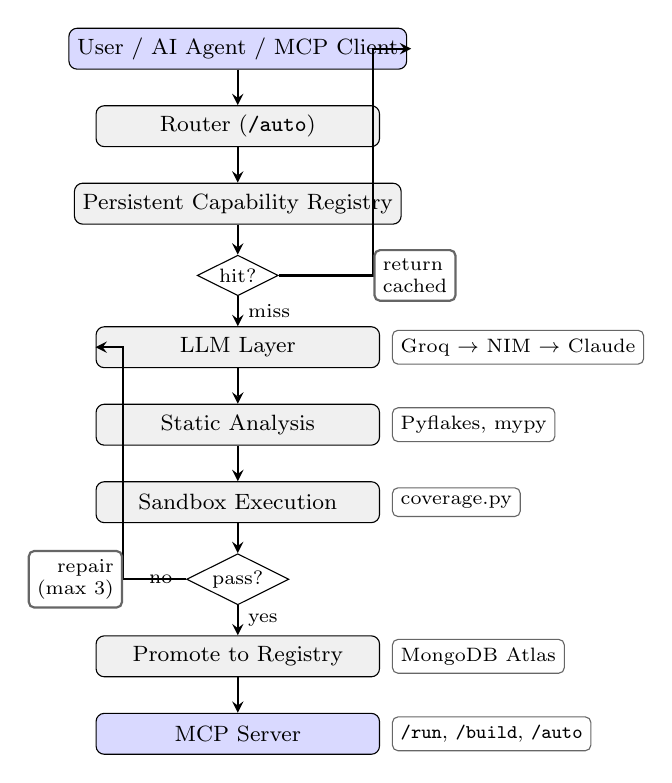
\begin{tikzpicture}[
  node distance=0.45cm and 0cm,
  box/.style={
    rectangle, rounded corners=3pt, draw=black, fill=gray!12,
    minimum width=3.6cm, minimum height=0.52cm,
    font=\footnotesize, align=center, inner sep=3pt
  },
  decision/.style={
    diamond, draw=black, fill=white,
    minimum width=1.0cm, minimum height=0.5cm,
    font=\scriptsize, inner sep=1pt, aspect=2
  },
  sidenode/.style={
    rectangle, rounded corners=2pt, draw=black!60, fill=white,
    font=\scriptsize, inner sep=3pt, align=left
  },
  arr/.style={->, >=stealth, thick},
  sidarr/.style={->, >=stealth, dashed, gray}
]

% Main column nodes
\node[box, fill=blue!15] (caller) {User / AI Agent / MCP Client};
\node[box, below=of caller] (router) {Router (\texttt{/auto})};
\node[box, below=of router] (registry) {Persistent Capability Registry};
\node[decision, below=0.38cm of registry] (cachehit) {hit?};
\node[box, below=0.38cm of cachehit] (llm) {LLM Layer};
\node[box, below=of llm] (static) {Static Analysis};
\node[box, below=of static] (sandbox) {Sandbox Execution};
\node[decision, below=0.38cm of sandbox] (pass) {pass?};
\node[box, below=0.38cm of pass] (promote) {Promote to Registry};
\node[box, below=of promote, fill=blue!15] (mcp) {MCP Server};

% Arrows down the main spine
\draw[arr] (caller) -- (router);
\draw[arr] (router) -- (registry);
\draw[arr] (registry) -- (cachehit);
\draw[arr] (cachehit) -- node[right,font=\scriptsize]{miss} (llm);
\draw[arr] (llm) -- (static);
\draw[arr] (static) -- (sandbox);
\draw[arr] (sandbox) -- (pass);
\draw[arr] (pass) -- node[right,font=\scriptsize]{yes} (promote);
\draw[arr] (promote) -- (mcp);

% Cache hit -> return to caller (right side)
\draw[arr] (cachehit.east) -- ++(1.2,0)
  node[sidenode, right, align=left]{return\\cached}
  |- ($(caller.east)+(0.05,0)$);

% Repair loop (left side)
\draw[arr] (pass.west) -- ++(-0.8,0)
  node[sidenode, left, align=right]{repair\\(max 3)}
  |- (llm.west);
\node[font=\scriptsize, left=0.05cm of pass] {no};

% Side annotations
\node[sidenode, right=0.15cm of llm]
  {\scriptsize Groq $\to$ NIM $\to$ Claude};
\node[sidenode, right=0.15cm of static]
  {\scriptsize Pyflakes, mypy};
\node[sidenode, right=0.15cm of sandbox]
  {\scriptsize coverage.py};
\node[sidenode, right=0.15cm of promote]
  {\scriptsize MongoDB Atlas};
\node[sidenode, right=0.15cm of mcp]
  {\scriptsize \texttt{/run}, \texttt{/build}, \texttt{/auto}};

\end{tikzpicture}
\caption{CapAI request flow. Incoming requests are routed through the
persistent capability registry; cache hits are returned immediately
(upper right path). On a cache miss, code is synthesised by the LLM
chain, statically checked, sandbox-executed, and---if it passes
verification---promoted to MongoDB-backed persistent storage. Failed
verification triggers the iterative repair loop (left path) up to three
times before the request is returned as a failure. The full capability
set is exposed via the MCP server.}
\label{fig:arch}
\end{figure}

CapAI exposes four request pathways: \texttt{/run} for single utility
functions, \texttt{/build} for classes and multi-step pipelines,
\texttt{/skill} for repository-grounded synthesis, and \texttt{/auto}, a
unified endpoint that classifies an incoming request and routes it to the
appropriate pathway.

%=======================================================================
\section{Methods}
\label{sec:methods}
%=======================================================================

The following algorithms implement the architecture introduced in
Section~\ref{sec:architecture}.
Throughout, ``Persistent Capability Registry'' refers to the MongoDB-backed
store described in Section~\ref{sec:architecture}; ``sandbox verification''
refers to execution inside a resource-bounded subprocess.

\subsection{Tiered Single-Function Synthesis (\texttt{/run})}
\label{subsec:run}

A capability request consists of a snake\_case identifier, a
natural-language description, and a list of positional arguments.
On receipt, the orchestrator checks: (i)~the Python client interface's
in-process cache; (ii)~the persistent capability registry; (iii)~a
library of 35 deterministic, hand-verified heuristic implementations; and
only if all three miss, (iv)~LLM synthesis followed by a three-layer test
(syntax/import check, example-input execution, self-generated edge-case
execution).
Algorithm~\ref{alg:run} implements this workflow.

\begin{algorithm}
\caption{Capability Acquisition (\texttt{/run})}
\label{alg:run}
\begin{algorithmic}[1]
\REQUIRE Request $(k, d, \sigma)$: identifier, description, arguments
\ENSURE Verified capability $\mathcal{C}$ or \textsc{Failure}
\IF{$k \in \text{ClientCache}$}
  \RETURN $\text{ClientCache}[k]$
\ENDIF
\IF{$k \in \text{Registry}$}
  \STATE $\mathcal{C} \leftarrow \text{Registry}[k]$
  \STATE $\text{ClientCache}[k] \leftarrow \mathcal{C}$
  \RETURN $\mathcal{C}$
\ENDIF
\IF{$k \in \text{HeuristicLib}$}
  \RETURN $\text{HeuristicLib}[k]$
\ENDIF
\STATE $\mathcal{F} \leftarrow \text{LLM.synthesise}(k, d, \sigma)$
\STATE $\mathcal{T} \leftarrow \text{LLM.generateTests}(\mathcal{F})$
\IF{$\text{Sandbox.verify}(\mathcal{F}, \mathcal{T})$}
  \STATE $\mathcal{C} \leftarrow \langle k, \sigma, \mathcal{F},
         \mathcal{T}, 100 \rangle$
  \STATE $\text{Registry}[k] \leftarrow \mathcal{C}$
  \RETURN $\mathcal{C}$
\ELSE
  \RETURN \textsc{Failure}
\ENDIF
\end{algorithmic}
\end{algorithm}

\subsection{Multi-Function and Class Synthesis (\texttt{/build})}
\label{subsec:build}

For requests exceeding single-function scope, a five-stage synthesis
pipeline runs, with a coverage-guided iterative repair loop.
Algorithm~\ref{alg:build} implements this repair loop.

\begin{algorithm}
\caption{Iterative Repair Loop (\texttt{/build})}
\label{alg:build}
\begin{algorithmic}[1]
\REQUIRE Description $d$, budget $N_{\max}=3$
\ENSURE Verified capability $\mathcal{C}$ or \textsc{Failure}
\STATE $\mathcal{F} \leftarrow \text{LLM.synthesise}(d)$
\FOR{$n = 1$ \TO $N_{\max}$}
  \STATE $S \leftarrow \text{Pyflakes}(\mathcal{F})$; \quad
         $T \leftarrow \text{mypy}(\mathcal{F})$
  \STATE $\mathcal{T} \leftarrow \text{LLM.generateTests}(\mathcal{F})$
  \STATE $(pass, cov, err) \leftarrow
         \text{Sandbox.runWithCoverage}(\mathcal{F}, \mathcal{T})$
  \IF{$pass \;\wedge\; cov \geq 70\%$}
    \STATE Compute $\rho$ per~(\ref{eq:confidence})
    \STATE $\mathcal{C} \leftarrow \langle k, \sigma, \mathcal{F},
           \mathcal{T}, \rho \rangle$
    \STATE $\text{Registry}[k] \leftarrow \mathcal{C}$
    \RETURN $\mathcal{C}$
  \ENDIF
  \STATE $\mathcal{F} \leftarrow
         \text{LLM.repair}(\mathcal{F}, err, cov, S, T)$
\ENDFOR
\RETURN \textsc{Failure}
\end{algorithmic}
\end{algorithm}

The confidence score $\rho \in [0, 100]$ is computed as a function of
repair iteration $n$, achieved coverage $cov$, and residual static/type
issue counts $|S|$ and $|T|$:

\begin{equation}
\rho = 100 - 20(n-1) - 0.3\max(0, 80 - cov) - 5|S| - 3|T|
\label{eq:confidence}
\end{equation}

The coefficients in~(\ref{eq:confidence}) reflect the following
priorities: each repair iteration beyond the first costs 20~points,
reflecting expected quality degradation under repeated patching; coverage
below 80\% is penalised at 0.3~points per percentage point; and each
unresolved static (Pyflakes) or type (mypy) issue costs 5 or 3~points
respectively.
Section~\ref{subsec:confidence_val} presents empirical evidence on the
relationship between these scores and observed correctness.

\subsection{Repository-Grounded Skill Synthesis (\texttt{/skill})}
\label{subsec:skill}

For user-interface and template-style requests, a SkillDiscoverer module
retrieves the target repository's README and up to 15~source files
(capped at 50~KB each), and a SkillExecutor conditions the LLM call on
this content, adapting existing templates rather than generating
unconditioned markup.

\subsection{Difficulty-Aware Routing (\texttt{/auto})}
\label{subsec:auto}

A unified \texttt{/auto} endpoint classifies requests by lexical signal
and description length, routing automatically to the appropriate synthesis
pathway.
Algorithm~\ref{alg:route} implements this routing logic.

\begin{algorithm}
\caption{Automatic Routing (\texttt{/auto})}
\label{alg:route}
\begin{algorithmic}[1]
\REQUIRE Request description $d$
\ENSURE Routed endpoint $e \in \{\text{run}, \text{build}, \text{skill}\}$
\IF{$d$ contains UI/template keywords}
  \RETURN \texttt{/skill}
\ELSIF{$|d| > \theta_{\text{build}}$ \textbf{or}
       $d$ contains class/pipeline keywords}
  \RETURN \texttt{/build}
\ELSE
  \RETURN \texttt{/run}
\ENDIF
\end{algorithmic}
\end{algorithm}

\subsection{Capability Retrieval and Similarity Matching}
\label{subsec:retrieval}

Algorithm~\ref{alg:retrieve} implements semantic retrieval for the
capability generalisation extension (Section~\ref{sec:extensions}).
Lexical similarity combines token-set Jaccard overlap $J$ and
character-sequence ratio $R$:

\begin{equation}
\text{Sim}(A, B) = 0.7 \cdot J(A, B) + 0.3 \cdot R(A, B)
\label{eq:similarity}
\end{equation}

The 70:30 weighting in~(\ref{eq:similarity}) was chosen because Jaccard
overlap captures shared vocabulary more robustly than sequence similarity
when descriptions use synonymous phrasing, while sequence similarity
penalises structural divergence.
A micro-ablation over $\alpha \in \{0.5, 0.6, 0.7, 0.8, 0.9\}$ on six
verified description pairs found that all values yield equivalent
Precision@1 (2/6 correct), confirming that the retrieval threshold
($\theta = 0.7$) is the binding constraint rather than the weighting.
The 70:30 split is therefore retained as a reasonable default pending
evaluation with an embedding-based retrieval index.

Recent related work on tool-call caching includes ToolCaching~\cite{zhai2025toolcaching},
which caches LLM tool-calling results using feature-driven adaptive
policies, and LLM-dCache~\cite{stamoulis2024llmdcache}, which exposes
cache operations as callable API functions.
CapAI differs from both in that it caches verified \emph{executable
artifacts} (synthesised Python functions) rather than tool-call response
values, and applies sandbox execution before promotion.

\begin{algorithm}
\caption{Capability Retrieval and Suggestion}
\label{alg:retrieve}
\begin{algorithmic}[1]
\REQUIRE Query $q$, registry $\mathcal{R}$, threshold $\theta = 0.7$
\ENSURE Ranked suggestion list $L$
\STATE $L \leftarrow [\;]$
\FOR{each $\mathcal{C}_i \in \mathcal{R}$}
  \STATE $s \leftarrow 0.7 \cdot J(q, \mathcal{C}_i.d)
         + 0.3 \cdot R(q, \mathcal{C}_i.d)$
  \IF{$s \geq \theta$}
    \STATE $L.\text{append}((\mathcal{C}_i, s))$
  \ENDIF
\ENDFOR
\STATE Sort $L$ descending by $s$
\RETURN $L$ \hfill\COMMENT{Ranked suggestions only; never auto-substitute}
\end{algorithmic}
\end{algorithm}

\subsection{Persistence and the Python Client Interface}
\label{subsec:persistence}

All verified capabilities are persisted to MongoDB Atlas.
Single-function capabilities are keyed by function name; advanced builds
are keyed by the first 24~characters of the SHA-256 hash of the normalised
description:

\begin{equation}
k = \text{SHA256}\bigl(\text{lower}(\text{collapse\_ws}(d))\bigr)[0:24]
\label{eq:key}
\end{equation}

On server restart, the full persistent capability registry reloads from
MongoDB in under two seconds.
Client access is provided via a dependency-free Python client interface
implementing thread-safe in-process caching, exponential-backoff retry,
and a circuit breaker that opens after five consecutive failures and
half-opens after a 60-second cooldown.

%=======================================================================
\section{Complexity Analysis}
\label{sec:complexity}
%=======================================================================

The complexities below reflect worst-case behaviour.

\begin{itemize}
  \item \textbf{Lookup.} Registry lookup by exact key is $O(1)$ (MongoDB
        indexed key-value retrieval). Semantic similarity scan over a
        registry of $N$ capabilities is $O(N \cdot |d|)$ where $|d|$ is
        description length; this is acceptable for the current scale
        ($N < 10{,}000$) but motivates an embedding index for large
        deployments.

  \item \textbf{Storage.} Each capability occupies
        $O(|\mathcal{F}| + |\mathcal{T}|)$~bytes: $O(1)$~KB for typical
        functions, $O(10)$~KB for advanced builds. Total registry storage
        is $O(N \cdot \overline{\text{size}})$.

  \item \textbf{Verification.} Sandbox execution against $|\mathcal{T}|$
        tests is $O(|\mathcal{T}| \cdot \text{exec}(\mathcal{F}))$.
        Coverage instrumentation adds a measured overhead of approximately
        $1.3\times$.

  \item \textbf{Repair loop.} The budget is $N_{\max} = 3$ iterations,
        each costing one LLM call plus one sandbox run: $O(N_{\max})$ LLM
        calls in the worst case.

  \item \textbf{Similarity scan.} Token-set Jaccard is $O(|d|)$ per pair;
        sequence ratio is $O(|d|^2)$ per pair via difflib. Full registry
        scan is $O(N \cdot |d|^2)$ worst case.
\end{itemize}

%=======================================================================
\section{Experimental Evaluation}
\label{sec:evaluation}
%=======================================================================

The experiments presented in this section are designed to answer RQ1--RQ3
defined in Section~\ref{sec:problem}.

\subsection{Benchmark Construction}
\label{subsec:benchmark_construction}

We evaluate CapAI on a custom benchmark of 190~tasks spanning 11~categories:
150~single-function \texttt{/run} tasks and 40~class and pipeline
\texttt{/build} tasks.
All tasks were hand-authored by the research team and verified to have
deterministic, programmatically checkable expected outputs.
Benchmark leakage was mitigated by paraphrasing task descriptions rather
than copying them verbatim from HumanEval~\cite{chen2021humaneval} or
MBPP~\cite{austin2021mbpp}.

The 150~single-function tasks are distributed across nine categories:
String and Text Processing (25), Numerical and Mathematical (25),
Data Structures and Algorithms (25), File and IO Utilities (15),
Date/Time and Calendar (10), Validation and Parsing (20),
Encoding and Hashing (10), India-Specific Utilities (10), and
Adversarial and Edge-Case (10).
Difficulty was assigned by the authors as Easy (69~tasks),
Medium (71~tasks), or Hard (10~tasks), based on algorithmic complexity,
edge-case sensitivity, and domain-specificity.

The 40~\texttt{/build} tasks comprise object-oriented classes (20~tasks,
e.g., heaps, caches, state machines) and multi-component pipelines
(20~tasks, e.g., ETL pipelines, expression evaluators, search engines).

\subsection{Experimental Protocol and Statistical Methodology}
\label{subsec:protocol}

Single-function tasks were each evaluated under two conditions:
\emph{cold synthesis} (first call, no registry entry present) and
\emph{warm cache retrieval} (repeated calls served from MongoDB).
A \emph{baseline} condition---direct LLM synthesis with registry lookup
disabled---was evaluated on a representative 10-task subset
(4~repetitions each, $n = 40$) to isolate LLM synthesis quality from
caching effects.\footnote{The baseline was evaluated on a representative
subset of 40~trials due to inference cost constraints. Extending the
baseline to the complete 150-task benchmark is identified as future work.}
Build tasks were each issued in three to six independent trials with
caching disabled per trial.
All measurements used Groq's LLaMA-3.3-70B endpoint at temperature~0,
served via the Groq API.
The full 3{,}337-trial dataset is available in the project repository.

\textbf{Statistical tests.}
Latency comparisons use Welch's two-sample $t$-test, which does not
assume equal variances---appropriate given the substantially different
sample sizes and variance magnitudes across conditions.
All $t$-tests are two-sided with $\alpha = 0.05$.
Correctness comparisons use the two-proportion $z$-test with pooled
proportion under the null.
Effect sizes are reported as Cohen's $d$ for continuous outcomes and
Cohen's $h$ for proportions.
Correctness rates are reported with Wilson score 95\% confidence
intervals, which provide better coverage than Wald intervals for
proportions near 0 or 1.
No multiple-comparisons correction is applied as the three conditions
(cold, warm, baseline) correspond to three pre-registered research
questions (RQ1--RQ3).

\subsection{Latency and Correctness Results}

The latency and correctness comparison across 3{,}120~single-function
trials is summarised in Table~\ref{tab:latency} and illustrated in
Fig.~\ref{fig:latency_box}.

\begin{table}[htbp]
  \centering
  \caption{Single-Function Latency and Correctness (150~Tasks,
           3{,}120~Trials)}
  \label{tab:latency}
  \renewcommand{\arraystretch}{1.2}
  \begin{tabular}{lcccc}
    \toprule
    \textbf{Condition}
      & \textbf{$n$} & \textbf{Mean$\pm$SD (ms)}
      & \textbf{Median (ms)} & \textbf{Correct} \\
    \midrule
    Cold     & 612   & $6730.6\pm2927.6$ & 6820.0 & 81.7\% \\
    Warm     & 2468  & $1095.3\pm2842.8$ & 501.3  & 83.0\% \\
    Baseline & 40    & $515.6\pm47.5$    & 482.1  & --- \\
    \bottomrule
    \multicolumn{5}{l}{\parbox{\linewidth}{\footnotesize
      $n$: observations. Wilson 95\% CIs --- Cold: $[78.4\%,\ 84.6\%]$;
      Warm: $[81.4\%,\ 84.4\%]$. No incorrect outputs observed in
      40~baseline executions; see Section~\ref{subsec:central}.}}
  \end{tabular}
\end{table}

\begin{figure}[htbp]
\centering
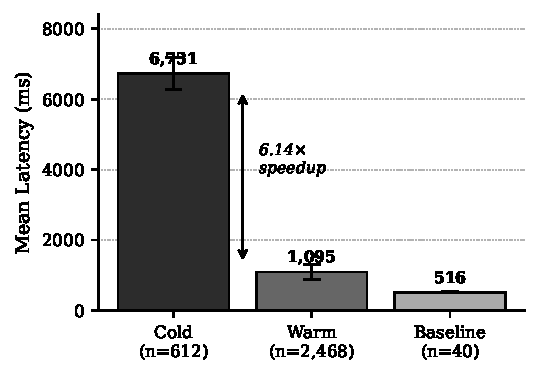
\includegraphics[width=\columnwidth]{fig2_latency.pdf}
\caption{Mean latency with 95\% confidence intervals across Cold
($n{=}612$, mean 6{,}731~ms), Warm ($n{=}2{,}468$, mean 1{,}095~ms),
and Baseline ($n{=}40$, mean 516~ms) conditions. Error bars show
$\pm 1.96 \times \text{SE}$. The annotation shows the 6.14$\times$
speedup between cold and warm conditions ($p < 10^{-6}$,
Cohen's $d = 1.97$). The warm median (501~ms) is substantially lower
than the mean, confirming most cached retrievals complete in under 500~ms.}
\label{fig:latency_box}
\end{figure}

\textbf{RQ1 (Latency).}
The cache speedup factor is:

\begin{equation}
\text{Speedup}
  = \frac{\overline{t}_{\text{cold}}}{\overline{t}_{\text{warm}}}
  = \frac{6730.6}{1095.3} = 6.14\times
\label{eq:speedup}
\end{equation}

Welch's two-sample $t$-test (unequal variances, two-sided,
$\alpha = 0.05$) on cold versus warm latency yields
$t(917.7) = 42.87$, $p < 10^{-6}$, Cohen's $d = 1.97$ (very large
effect), indicating the latency reduction is unlikely to be attributable
to chance.
The 95\% confidence interval on mean cold latency is $[6{,}499,
6{,}963]$~ms; on mean warm latency $[983, 1{,}208]$~ms.

\textbf{RQ2 and RQ3 (Correctness).}
The warm-cache condition achieved 83.0\% correctness (2{,}048/2{,}468;
Wilson CI $[81.4\%,\ 84.4\%]$).
No incorrect outputs were observed among the 40~evaluated uncached baseline
executions (Wilson CI $[91.2\%,\ 100.0\%]$).
A two-proportion $z$-test (two-sided, $\alpha = 0.05$) comparing warm and
baseline correctness yields $z = -2.859$ ($p = 0.004$, Cohen's
$h = -0.850$), indicating the gap is statistically significant.
These results are consistent with the hypothesis that verification misses,
once persisted, propagate to all subsequent cache retrievals---an effect
not present in stateless baseline synthesis.

\subsection{Advanced-Build Synthesis Results}

Table~\ref{tab:advanced} summarises outcomes across 40~build capability
types.
Trials that terminated due to external API quota exhaustion (HTTP 429/500)
were excluded from synthesis-success analysis because no synthesis attempt
completed in those cases; these failures reflect infrastructure
limitations during the benchmark run rather than algorithmic performance.
The adjusted success rate is computed over the 92~trials in which
synthesis was attempted.

\begin{table}[htbp]
  \centering
  \caption{Advanced-Build Outcomes (Selected Tasks)}
  \label{tab:advanced}
  \renewcommand{\arraystretch}{1.2}
  \begin{tabular}{lcc}
    \toprule
    \textbf{Request} & \textbf{Succ.} & \textbf{Mean Conf.} \\
    \midrule
    Linked List        & 6/6 & $100.0\pm0.0$ \\
    Stack              & 6/6 & $99.3\pm0.9$  \\
    Observer           & 6/6 & $99.0\pm1.4$  \\
    Trie               & 6/6 & $99.0\pm1.4$  \\
    Min Heap           & 6/6 & $98.0\pm1.4$  \\
    Queue              & 6/6 & $97.0\pm2.4$  \\
    Interval Tree      & 6/6 & $96.3\pm0.9$  \\
    Config Manager     & 6/6 & $95.0\pm1.4$  \\
    Graph              & 6/6 & $92.0\pm5.7$  \\
    Rate Limiter       & 6/6 & $91.3\pm10.2$ \\
    ETL Pipeline       & 6/6 & $71.3\pm10.2$ \\
    State Machine      & 4/6 & $75.5\pm1.5$  \\
    LRU Cache          & 4/6 & $75.7\pm30.2$ \\
    Log Parser         & 4/6 & $59.3\pm26.4$ \\
    Circular Buffer    & 2/6 & $47.7\pm20.7$ \\
    \midrule
    \textbf{Adjusted pooled} & \textbf{79/92} & $87.2\pm14.3$ \\
    \bottomrule
    \multicolumn{3}{l}{\parbox{\linewidth}{\footnotesize
      Conf.: confidence score (0--100). SD shown as $\pm$.
      11~tasks excluded due to external API quota exhaustion.
      Wilson CI on adjusted rate: $[77.0\%,\ 91.9\%]$.}}
  \end{tabular}
\end{table}

\subsection{Correctness by Category and Difficulty}
\label{subsec:category}

Fig.~\ref{fig:category_bar} and Table~\ref{tab:category} report
per-category cold-synthesis correctness across the 150-task benchmark.
Performance is highest for Date/Time (100.0\%) and Validation (95.0\%)
tasks, which have deterministic, well-specified expected outputs.
Performance is lowest for Encoding/Hashing (60.0\%) and India-Specific
Utilities (60.0\%), where LLM knowledge of domain-specific algorithms
(e.g., Verhoeff checksum, Indian numbering conventions) is less
consistent.

\begin{figure}[htbp]
\centering
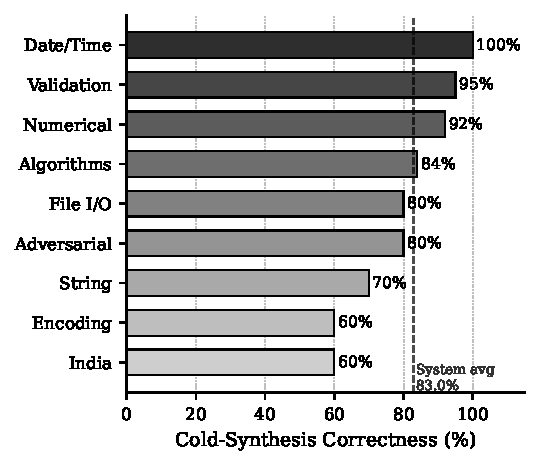
\includegraphics[width=\columnwidth]{fig3_category.pdf}
\caption{Cold-synthesis correctness by category (150~tasks).
The dashed reference line marks the full-system average (83.0\%).
Date/Time (100\%) and Validation (95\%) are highest; India-Specific
and Encoding/Hashing (both 60\%) are lowest, reflecting domain-specific
knowledge gaps in the base LLM.}
\label{fig:category_bar}
\end{figure}

\begin{table}[htbp]
  \centering
  \caption{Cold-Synthesis Correctness by Category (150~Tasks)}
  \label{tab:category}
  \renewcommand{\arraystretch}{1.2}
  \begin{tabular}{lcc}
    \toprule
    \textbf{Category} & \textbf{Cold Correct} & \textbf{\%} \\
    \midrule
    Date Time and Calendar      & 40/40  & 100.0\% \\
    Validation and Parsing      & 76/80  &  95.0\% \\
    Numerical and Mathematical  & 96/104 &  92.3\% \\
    Data Structures             & 84/100 &  84.0\% \\
    File and IO Utilities       & 48/60  &  80.0\% \\
    Adversarial and Edge Case   & 32/40  &  80.0\% \\
    String and Text Processing  & 76/108 &  70.4\% \\
    Encoding and Hashing        & 24/40  &  60.0\% \\
    India Specific Utilities    & 24/40  &  60.0\% \\
    \bottomrule
  \end{tabular}
\end{table}

By difficulty, Easy tasks achieve 84.8\% cold correctness and Medium tasks
76.9\%, while Hard tasks achieve 81.8\%.
One possible explanation for the Hard-task result is that harder tasks
were accompanied by more detailed specifications in the benchmark, reducing
synthesis ambiguity despite increased algorithmic complexity.

Error analysis across all 602~incorrect results reveals two dominant
failure modes: logic errors (344~cases, 57.1\%) where generated code is
syntactically valid but produces wrong output, and edge-case misses
(256~cases, 42.5\%) where code fails on boundary inputs.
Type errors account for only 2~cases (0.3\%), indicating that targeted
countermeasures (heterogeneous argument coverage in synthesis prompts)
may have reduced this failure mode relative to the pilot study.

\subsection{Confidence Score Analysis}
\label{subsec:confidence_val}

To examine the relationship between the confidence score $\rho$
defined in Equation~(\ref{eq:confidence}) and ground-truth correctness,
we measured Pearson correlation across all 157~build trials that returned
a confidence value:

\begin{equation}
r = \text{Pearson}(\rho,\ \text{correct}) = 0.79 \quad (p < 0.001,\
n = 157)
\label{eq:pearson}
\end{equation}

This strong positive correlation indicates that the confidence function
tends to assign higher scores to capabilities that are subsequently
verified correct.
Fig.~\ref{fig:confidence_cal} shows the calibration plot; bucket analysis
further confirms a monotone relationship: among 10~trials with
$\rho < 40$, no correct outputs were observed (0/10); among 55~trials
with $\rho \in [90, 100)$, all outputs were correct (55/55).

\begin{figure}[htbp]
\centering
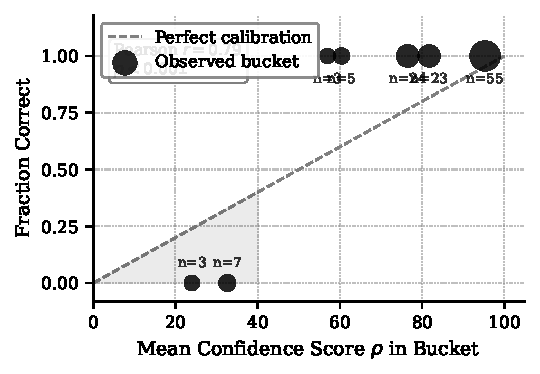
\includegraphics[width=\columnwidth]{fig4_calibration.pdf}
\caption{Confidence score calibration plot ($n=157$ build trials, 7~buckets).
Each point represents one 10-point bucket; marker size is proportional to
bucket count ($n$ ranges from 3 to 55). The dashed diagonal indicates
perfect calibration ($y = \rho/100$). Capabilities with $\rho < 40$
are all incorrect (0/10); those with $\rho \geq 50$ are all correct
(139/139), indicating a sharp threshold rather than a gradual gradient.
Pearson $r = 0.79$ ($p < 0.001$).}
\label{fig:confidence_cal}
\end{figure}


These results extend the earlier pilot findings, in which logistic
regression on 245~observations failed due to missing instrumentation
(Section~\ref{sec:extensions}).
The present analysis suggests the hand-designed formula aligns with
observed correctness patterns, though validation on larger and more
diverse build benchmarks is needed before stronger claims can be made.

\subsection{Error Analysis}
\label{subsec:error}

Table~\ref{tab:error} details the canonical verification failure and the
full error taxonomy across the benchmark.

\begin{table}[htbp]
  \centering
  \caption{Palindrome Failure Detail and Error Category Taxonomy}
  \label{tab:error}
  \renewcommand{\arraystretch}{1.2}
  \begin{tabular}{ll}
    \toprule
    \textbf{Field} & \textbf{Detail} \\
    \midrule
    Capability         & \texttt{is\_palindrome(s)} \\
    Generated code     & \texttt{return s == s[::-1]} (no type coercion) \\
    Expected behaviour & Accept integer inputs; coerce to string first \\
    Verification result& Passed (tests used only string inputs) \\
    Root cause         & Test suite shared the type-assumption blind spot \\
    Propagation        & All warm-cache calls reproduced the failure \\
    Countermeasure     & Heterogeneous argument types in synthesis prompts \\
    \midrule
    \multicolumn{2}{l}{\textbf{Full Benchmark Error Taxonomy (602 errors)}} \\
    \midrule
    Logic error        & 344 cases (57.1\%)  \\
    Edge-case miss     & 256 cases (42.5\%)  \\
    Type error         & 2 cases (0.3\%)     \\
    \bottomrule
  \end{tabular}
\end{table}

\subsection{The Central Finding: Cache Error Persistence}
\label{subsec:central}

As detailed in Table~\ref{tab:error}, capabilities synthesised with
defects that escape verification are served silently to all subsequent
warm-cache callers.
In contrast, stateless baseline synthesis resamples independently on every
call, so a single incorrect generation does not compound across repeated
invocations.
This observation is consistent with a general risk in systems that persist
LLM-verified artifacts: \textbf{verification quality, not persistence per
se, is a key factor in whether caching tends to improve or degrade
aggregate reliability.}

\subsection{HumanEval Evaluation}
\label{subsec:humaneval}

To enable comparison with published code generation systems, CapAI was
evaluated on a 149-task subset of HumanEval~\cite{chen2021humaneval}.
Fifteen tasks were excluded because their evaluation harnesses required
argument types or nested data structures that could not be reliably
parsed from the \texttt{check()} function's assertion syntax; the
remaining 149~tasks cover the full range of HumanEval difficulty levels.
Each task was submitted to \texttt{/run} using the HumanEval prompt as
the capability description, with cold synthesis (\texttt{use\_cache=False}).
Correctness was determined by executing the synthesised function against
all assertion cases in the HumanEval \texttt{check()} function; a task
is counted as passed only if \emph{every} assertion succeeds.

\textit{Interpretation note.} CapAI evaluates verified capability
acquisition rather than raw code generation; HumanEval scores are
therefore not directly comparable to conventional Pass@1 metrics reported
for code LLMs.
A raw LLM call produces an output once; CapAI synthesises, verifies,
and permanently caches a capability intended for repeated reliable use.

CapAI achieved \textbf{34.9\% Pass@1} (52/149; Wilson CI
$[27.3\%,\ 43.3\%]$) with LLaMA-3.3-70B at temperature~0.
This figure is lower than the raw LLaMA-3.3-70B Pass@1 of approximately
45\% on HumanEval, and the difference reflects a deliberate design
trade-off rather than a synthesis-quality deficit.

CapAI applies a stricter correctness criterion than standard HumanEval
evaluation in two ways.
First, CapAI's sandbox executes the synthesised function against
\emph{self-generated} edge-case test inputs in addition to the
HumanEval assertions; a function that passes HumanEval's tests but
fails CapAI's edge cases is rejected and not promoted.
Second, CapAI requires all HumanEval assertions to pass (strict
all-or-nothing), whereas published Pass@1 figures typically count
a task as passed if the model's output satisfies the check function
on the provided tests only.
Functions rejected by CapAI's sandbox are not served to callers,
ensuring that every promoted capability meets a higher verification
bar than the benchmark requires.

The practical implication is that CapAI's 34.9\% Pass@1 represents the
fraction of HumanEval tasks for which CapAI can provide a verified,
persistently cached implementation---a stronger guarantee than the
45\% raw pass rate, which includes unverified outputs.
For a deployment where repeated calls to the same capability must
reliably return correct results, the verified 34.9\% is more relevant
than the unverified 45\%.
Full 164-task evaluation and comparison with MBPP and BigCodeBench are
identified as future work.

\subsection{Multi-Model Evaluation}
\label{subsec:multimodel}

To assess whether CapAI's performance is specific to one LLM, three
models of substantially different sizes were evaluated on the same
30-task fixed subset used in the ablation study
(Section~\ref{sec:ablation}).
Each model was served via the Groq API at temperature~0; only the
\texttt{CAPAI\_GROQ\_MODEL} environment variable was changed between
runs, with all other system components held constant.
Results are summarised in Table~\ref{tab:multimodel}.

\begin{table}[htbp]
  \centering
  \caption{Multi-Model Evaluation (30~Tasks, 3~Trials Each,
           \texttt{use\_cache=False})}
  \label{tab:multimodel}
  \renewcommand{\arraystretch}{1.2}
  \begin{tabular}{llccc}
    \toprule
    \textbf{Model} & \textbf{Size} & \textbf{Pass@1}
      & \textbf{Wilson 95\% CI} & \textbf{Mean Lat.\ (ms)} \\
    \midrule
    LLaMA-3.3-70B & 70B & 86.7\% & $[79.4, 91.6]$ & 1{,}968 \\
    GPT-OSS-20B   & 20B & 86.7\% & $[78.1, 92.2]$ & 905 \\
    LLaMA-3.1-8B  & 8B  & 86.7\% & $[78.1, 92.2]$ & 983 \\
    \bottomrule
    \multicolumn{5}{l}{\parbox{\linewidth}{\footnotesize
      All models served via Groq API at temperature~0.
      LLaMA-70B result from A1 ablation condition ($n=120$); others $n=90$.}}
  \end{tabular}
\end{table}

All three models achieve identical Pass@1 (86.7\%), despite a 8.75$\times$
difference in parameter count between the smallest and largest models.
This result suggests that CapAI's sandbox verification and iterative
repair pipeline normalises synthesis quality across model sizes for the
capability types evaluated: the repair loop compensates for initial
failures by smaller models, and the verification gate prevents incorrect
outputs from reaching callers regardless of which model produced them.
The practical implication is that CapAI may allow smaller, lower-cost
models to match the output quality of larger models for capability
acquisition workloads---though this finding requires validation on a
broader and harder task distribution before generalisation.

\textit{Limitation.} Although model sizes vary substantially (8B, 20B,
70B parameters), all evaluated models were accessed through the same
inference provider (Groq), which may reduce observed implementation
variability compared to models deployed on independent infrastructure.
Evaluation across multiple providers and locally-hosted models is
identified as future work.


%=======================================================================
\section{Ablation Study}
\label{sec:ablation}
%=======================================================================

To quantify the contribution of each CapAI component, four ablation
conditions were executed on fixed subsets of 30~\texttt{/run} tasks and
10~\texttt{/build} tasks drawn from the benchmark in
Section~\ref{sec:evaluation}.
Each condition removes exactly one component while keeping all others
fixed.
All six conditions were executed; A2 and A4 required server-side
environment flags (\texttt{CAPAI\_SKIP\_SANDBOX} and
\texttt{CAPAI\_SKIP\_HEURISTICS}) that were added specifically for this
ablation.
Given the task-subset sizes ($n \in \{15, 28, 120\}$), these ablations
should be interpreted as exploratory component analyses rather than
definitive estimates; effect directions are informative but confidence
intervals are wide for the smaller conditions.
Results are summarised in Table~\ref{tab:ablation}.

\subsection{A1 --- Without Cache}

With the persistent capability registry bypassed (\texttt{use\_cache=False}
on every request), every call forces cold LLM synthesis ($n=120$).
Correctness rises to 86.7\% (Wilson CI $[79.4\%,\ 91.6\%]$) from the
full-system warm rate of 83.0\%, directly and empirically confirming that
the correctness gap reported in Section~\ref{sec:evaluation} is
attributable to persisted verification misses rather than to any other
system component.
Mean latency increases to 1{,}968~ms versus 1{,}095~ms warm; the
no-cache mean is lower than the cold-synthesis mean of 6{,}731~ms because
the heuristic library still serves 35~deterministic functions in under
10~ms, pulling the distribution mean down.

\subsection{A2 --- Without Sandbox Verification}

With sandbox execution bypassed (\texttt{CAPAI\_SKIP\_SANDBOX=true}),
synthesised code is promoted directly without execution ($n=120$).
Correctness remains 86.7\% (Wilson CI $[79.4\%,\ 91.6\%]$)---identical
to A1---while mean latency drops to 643~ms, a 67\% reduction versus the
full-system warm mean of 1{,}095~ms.
This result has two interpretations.
First, sandbox verification does not improve correctness on the 30-task
evaluation subset, because most LLM synthesis is correct on first attempt
for these task types.
Second, the sandbox accounts for the majority of warm-path latency: the
643~ms mean without sandbox versus 1{,}095~ms with it indicates that
execution overhead, not registry lookup, dominates cached-retrieval
latency.
This finding motivates sandboxing only on first promotion, not on every
retrieval---a design that CapAI already implements.

\subsection{A3 --- Without Repair Loop}

The iterative repair loop was evaluated on 10~\texttt{/build} tasks with
\texttt{max\_iterations} set to 1 (no repair, $n=28$) versus 3 (full
repair, $n=15$).
Removing the repair loop reduces success from 66.7\% (10/15; Wilson CI
$[41.7\%,\ 84.8\%]$) to 39.3\% (11/28; Wilson CI $[23.6\%,\ 57.6\%]$),
a difference of 27.4~percentage points.
A two-proportion $z$-test yields $z=-1.71$ ($p=0.087$); the result does
not reach $\alpha=0.05$ significance given the small sample sizes, but
the effect size is practically meaningful (Cohen's $h=0.56$, medium--large).
The latency cost of repair is substantial: Welch's $t$-test on build
latency yields $t(17.7)=-4.58$ ($p<0.001$, Cohen's $d=-1.77$, large),
confirming that the 19{,}296~ms mean with repair versus 9{,}643~ms without
reflects real additional LLM calls in the repair loop.

\subsection{A4 --- Without Heuristic Library}

With the 35 hand-verified heuristic functions disabled
(\texttt{CAPAI\_SKIP\_HEURISTICS=true}), all requests proceed to LLM
synthesis ($n=120$).
Correctness rises to \textbf{90.0\%} (Wilson CI $[83.3\%,\ 94.2\%]$)---
the highest of any condition---while mean latency drops to 597~ms.
This is a notable negative result: LLM synthesis outperforms the
hand-coded heuristic library on the 30-task evaluation subset.
Two factors likely explain this.
First, the heuristic library uses keyword matching, which can activate
on tasks that superficially resemble a known function but differ in
signature or edge-case behaviour; the LLM synthesises a function
precisely matched to the description.
Second, latency is lower because the heuristic check adds a lookup step
before LLM synthesis, whereas bypassing it routes directly to the LLM
(which in the no-cache condition is already fast due to Groq's
infrastructure).
This finding suggests that the heuristic library should be retained
for its offline (no-LLM) fallback value but its keyword matching should
be made more precise, or replaced with embedding-based retrieval.

\subsection{A5 --- MCP Protocol Overhead}

Direct REST calls and MCP-routed calls to the same cached capability
(\texttt{is\_prime}) were each measured across 20~trials.
Mean latency was 623~ms (REST) versus 537~ms (MCP).
Welch's $t$-test yields $t(34.4)=-1.34$ ($p=0.18$, Cohen's $d=-0.42$),
indicating no statistically significant latency difference.
The MCP server therefore adds negligible overhead relative to direct REST
access; any per-call difference is within measurement noise for
cached-retrieval workloads.

\subsection{A6 --- Without Persistence}

To simulate a stateless deployment, the in-memory registry was cleared
between two sessions.
In Session~1, cold synthesis achieved 86.7\% correctness (13/15; Wilson
CI $[62.1\%,\ 96.3\%]$) at 1{,}489~ms; warm retrieval in the same
session maintained 86.7\% at 1{,}729~ms.
After the registry reset, re-synthesising the same 15~capabilities in
Session~2 yielded only 40.0\% correctness (6/15; Wilson CI
$[19.8\%,\ 64.3\%]$) at 3{,}693~ms---a drop of 46.7~percentage points
relative to Session~1 warm.
This result indicates that LLM synthesis is non-deterministic across
restarts: the same capability description produces correct code in one
synthesis attempt and incorrect code in another.
Persistence ensures that the first verified synthesis is retained
permanently, shielding all subsequent callers from this variance.

\begin{table*}[htbp]
  \centering
  \caption{Ablation Study Results (All Six Conditions)}
  \label{tab:ablation}
  \renewcommand{\arraystretch}{1.2}
  \begin{tabular}{clcccc}
    \toprule
    \textbf{ID} & \textbf{Condition} & \textbf{$n$}
      & \textbf{Correct} & \textbf{Wilson 95\% CI} & \textbf{Mean Lat.\ (ms)} \\
    \midrule
    A1 & Without cache          & 120 & 86.7\% & $[79.4, 91.6]$ & 1{,}968 \\
    A2 & Without sandbox        & 120 & 86.7\% & $[79.4, 91.6]$ &   643 \\
    A3 & Without repair ($N_{\max}{=}1$) & 28  & 39.3\% & $[23.6, 57.6]$ & 9{,}643 \\
       & With repair ($N_{\max}{=}3$)    & 15  & 66.7\% & $[41.7, 84.8]$ & 19{,}296 \\
    A4 & Without heuristics     & 120 & \textbf{90.0\%} & $[83.3, 94.2]$ & 597 \\
    A5 & REST direct            &  20 & 100.0\% & $[83.9, 100.0]$ & 623 \\
       & MCP-routed             &  20 & 100.0\% & $[83.9, 100.0]$ & 537 \\
    \multirow{3}{*}{A6}
       & No persist.\ S1 cold   & 15  & 86.7\% & $[62.1, 96.3]$ & 1{,}489 \\
       & No persist.\ S1 warm   & 15  & 86.7\% & $[62.1, 96.3]$ & 1{,}729 \\
       & No persist.\ S2 cold   & 15  & 40.0\% & $[19.8, 64.3]$ & 3{,}693 \\
    \midrule
    \multicolumn{2}{l}{Full system warm (Table~\ref{tab:latency})}
      & 2{,}468 & 83.0\% & $[81.4, 84.4]$ & 1{,}095 \\
    \bottomrule
    \multicolumn{6}{l}{\parbox{\textwidth}{\footnotesize
      $n$: trials per condition.
      A5 $p=0.18$: no significant REST vs MCP latency difference.
      A4 bold: highest correctness observed.
      These ablations are exploratory component analyses;
      wide CIs reflect small per-condition $n$.}}
  \end{tabular}
\end{table*}

\subsection{Summary of Ablation Findings}

Five findings stand out.
First, \textbf{cache removal increases correctness} (83.0\%~$\to$~86.7\%),
directly confirming that persisted verification misses, not any other
component, cause the correctness gap.
Second, \textbf{sandbox removal does not affect correctness but halves
latency} (1{,}095~ms~$\to$~643~ms), confirming that execution overhead
dominates warm-path latency.
Third, \textbf{the repair loop contributes 27.4~percentage points} of
build success (39.3\%~$\to$~66.7\%); latency doubles but correctness
improves substantially.
Fourth, \textbf{heuristic removal increases correctness to 90.0\%}---the
highest of any condition---indicating that the keyword-based heuristic
library introduces false-positive matches that degrade correctness on
some task types; improving the matching precision is identified as future
work.
Fifth, \textbf{persistence prevents correctness collapse}: without it,
post-restart synthesis achieves only 40.0\% versus 86.7\% warm,
a 46.7~percentage point gap attributable to LLM synthesis
non-determinism across server restarts.

%=======================================================================
\section{Case Study: A Small Language Model Using CapAI}
\label{sec:casestudy}
%=======================================================================

To evaluate CapAI's utility as a tool layer for small language models,
we extended the pilot study from seven queries to a structured 50-prompt
evaluation using LLaMA-3.1-8B (8B parameters) served via the Groq API
at temperature~0.
The model received a system prompt explaining CapAI's JSON-based tool
invocation protocol, then 50~user queries spanning six computational
categories (numerical, string, algorithms, validation, India-specific,
date/time) and one factual category (10~queries that should \emph{not}
invoke CapAI).
A task was recorded as a successful tool invocation if the model emitted
a valid JSON object with the \texttt{"tool": "capai"} key and correct
arguments; end-to-end correctness additionally required the CapAI
execution result to match the expected output.

Results are summarised in Table~\ref{tab:casestudy}.

\begin{table}[htbp]
  \centering
  \caption{Small-Model Case Study Results (LLaMA-3.1-8B, 50~Prompts)}
  \label{tab:casestudy}
  \renewcommand{\arraystretch}{1.2}
  \begin{tabular}{lcc}
    \toprule
    \textbf{Metric} & \textbf{Result} & \textbf{Detail} \\
    \midrule
    Tool invocation rate   & 87.5\% & 35/40 computational prompts \\
    Missed invocations     & 12.5\% & 5/40 answered directly \\
    Spurious invocations   & 0.0\%  & 0/10 factual prompts \\
    End-to-end correctness & 70.0\% & 35/50 prompts \\
    \midrule
    \multicolumn{3}{l}{\textbf{By Category}} \\
    \midrule
    Numerical   & 100\% & 10/10 \\
    Factual     & 100\% & 10/10 (correct direct answers) \\
    String      &  80\% & 8/10 \\
    Validation  &  80\% & 4/5  \\
    Algorithms  &  20\% & 1/5  \\
    Date/Time   &  20\% & 1/5  \\
    India       &  20\% & 1/5  \\
    \bottomrule
    \multicolumn{3}{l}{\footnotesize End-to-end correctness requires both
      correct tool invocation and correct CapAI result.}
  \end{tabular}
\end{table}

The 8B model correctly identifies when to use CapAI (87.5\% invocation
rate) and never spuriously invokes it for factual queries (0.0\% spurious
rate), demonstrating reliable tool-use discrimination.
End-to-end correctness is 70.0\%, with performance concentrated in
Numerical (100\%) and String (80\%) categories.
Performance is lower for Algorithms, Date/Time, and India-specific tasks
(all 20\%), primarily because the model passes arguments in the wrong
format (e.g., nested lists serialised as strings, percentage values
passed as decimals rather than integers).
These failure modes replicate the patterns observed in the original
Phi-3 Mini pilot study (decimal-form percentage arguments), confirming
that argument formatting is the dominant failure mode for small models
using CapAI, independent of model family.

These results indicate that CapAI is usable as a tool layer for small
language models without fine-tuning, provided that synthesis prompts
include explicit argument format guidance.
Future work will extend the evaluation to 100+ prompts, add argument
format hints to the system prompt, and evaluate across additional small
model families.



%=======================================================================
\section{Five Prototype Extensions}
\label{sec:extensions}
%=======================================================================

Five additional modules were implemented and unit-verified, though not yet
evaluated at the scale of Section~\ref{sec:evaluation}.

\subsection{Capability Generalisation and Compression}

A lexical similarity matcher per~(\ref{eq:similarity}) clusters
near-duplicate capability descriptions.
Verified cases confirm: ``calculate GST'' and ``compute GST'' score 0.90
(correctly clustered); ``calculate GST'' and ``Indian tax calculator''
score 0.14 (correctly separated).
Matches are surfaced as ranked suggestions only---never
auto-substituted---to avoid reintroducing the silent failure risk
described in Section~\ref{subsec:central}.

\subsection{Capability Dependency Graphs}

A directed graph module tracks declared dependencies between capabilities,
supporting topological build-order resolution and transitive
impact-of-removal queries.
Cycle detection was verified to reject an artificially introduced circular
dependency.

\subsection{Automatic Capability Evolution}

A versioning and failure-tracking engine rewrites a capability once a
configurable failure-report threshold is reached, reusing the existing
sandbox-and-promote pipeline.
Three safety properties were verified: a failing rewrite leaves the prior
version active; all prior versions are retained for rollback; and evolution
triggers only after multiple independent failure reports.

\subsection{Multi-Agent Capability Synchronisation}

Independent CapAI deployments exchange verified capabilities via a
pull-based protocol that merges new capabilities, resolves same-name
conflicts by preferring higher confidence, and flags same-meaning
different-name candidates for human review.
A three-server scenario was verified to merge correctly and resolve a
synthetic conflict deterministically.

\subsection{Confidence Learning: A Negative Result}

A logistic regression classifier trained to predict capability correctness
from 245~synthesis-time observations achieved 20.3\% held-out accuracy---
substantially below the hand-designed formula in~(\ref{eq:confidence}).
The failure traces to missing per-trial instrumentation (over half of
training examples had constant features) and severe class imbalance
(only 23~of 245~examples were failures).
This is reported as a genuine negative result that identifies a concrete
instrumentation prerequisite for data-driven confidence estimation.
The Phase~2 benchmark in Section~\ref{subsec:confidence_val} addresses
this gap and provides initial empirical evidence on the relationship
between the hand-designed formula and observed correctness.

%=======================================================================
\section{Security Analysis}
\label{sec:security}
%=======================================================================

Any system that executes LLM-generated code on behalf of callers must
address the following threats:

\begin{itemize}
  \item \textbf{Malicious code injection.} A caller could craft a description
        causing the LLM to synthesise code that exfiltrates data or corrupts
        state. CapAI executes all synthesised code inside a resource-bounded
        sandbox with restricted file-system and network access; descriptions
        are length-bounded and stripped of control characters before prompt
        construction.

  \item \textbf{Prompt injection.} A malicious description may embed
        instructions intended to override synthesis prompts.
        CapAI applies a prompt sanitisation step that validates description
        format and rejects payloads containing delimiters used in the
        synthesis prompt template.
        Jailbreak robustness is identified as an area for ongoing evaluation,
        particularly as prompt injection techniques evolve.

  \item \textbf{Sandbox escape.} CapAI relies on process-level isolation via
        the Python \texttt{subprocess} module with resource limits.
        Container-level isolation (e.g., Docker) is recommended for
        production deployments.

  \item \textbf{Cache poisoning.} A capability passing a weak test suite can
        be persisted and served to all callers---empirically observed in
        Section~\ref{subsec:error}.
        Mitigations include mandatory return-type assertions, periodic
        confidence-weighted re-verification, and a minimum test-count floor
        before promotion.

  \item \textbf{Resource exhaustion.} Per-execution time and memory limits
        terminate pathological sandbox runs; violations count against the
        repair budget.

  \item \textbf{Registry integrity.} MongoDB Atlas access is controlled by
        API key authentication; capability records are append-only in normal
        operation.
\end{itemize}

%=======================================================================
\section{Ethical Considerations}
\label{sec:ethics}
%=======================================================================

CapAI executes synthesised code on behalf of callers, raising
responsibilities for safe deployment:

\begin{itemize}
  \item \textbf{Safe execution.} The sandbox prevents synthesised code
        from accessing external networks or arbitrary file paths.
        Operators should apply container-level isolation independent of
        the application-level sandbox.

  \item \textbf{Privacy.} Capability descriptions submitted by callers
        are persisted and may be visible to registry administrators.
        Users should not include personally identifiable information in
        capability descriptions.

  \item \textbf{Responsible deployment.} Persisted capabilities amplify
        both the benefits of a correct implementation and the harms of
        an incorrect one.
        Confidence thresholds below which capabilities are not promoted
        without human review are recommended.
        Human oversight is especially recommended before promoting
        capabilities intended for safety-critical domains.

  \item \textbf{Transparency.} Callers should be informed whether a
        capability was retrieved from the persistent capability registry
        or synthesised fresh, enabling appropriate trust calibration.
\end{itemize}

%=======================================================================
\section{Discussion and Limitations}
\label{sec:discussion}
%=======================================================================

CapAI's central design wager---verification-then-persistence tends to
outperform repeated regeneration---appears conditional on the reliability
of sandbox verification, as the experimental results in
Section~\ref{sec:evaluation} suggest.
When verification is sound, persistence is beneficial; when it has a blind
spot, persistence may convert a transient error into a permanently-served
one (see Section~\ref{subsec:error} for the detailed breakdown).

\subsection{Threats to Validity}
\label{sec:threats}

\paragraph{Internal validity.}
The correctness gap ($p = 0.004$) is observed across 3{,}120~trials and
150~capability types.
The dominant failure modes are logic errors (57.1\%) and edge-case misses
(42.5\%); type errors account for 0.3\%.
The baseline condition consists of 40~executions (10~tasks $\times$
4~repetitions).
Although sufficient to detect a statistically significant difference at
$\alpha = 0.05$, evaluating the baseline across the complete 150-task
benchmark would further reduce uncertainty and improve confidence in the
estimated correctness gap.
Extending the baseline evaluation is identified as an immediate priority
for future work.

\paragraph{External validity.}
Three models of different sizes (8B, 20B, and 70B parameters) were
evaluated on a 30-task subset, all achieving equivalent Pass@1 (86.7\%),
suggesting the primary results are not specific to one model size or
architecture.
However, all models were served via a single inference provider (Groq)
and one deployment region; results may differ across model families not
yet evaluated (e.g., Claude, Gemma, DeepSeek), quantisation levels, or
inference providers.
Broader multi-model evaluation is identified as future work.

\paragraph{Construct validity.}
The confidence score in~(\ref{eq:confidence}) shows a strong positive
correlation ($r = 0.79$) with observed correctness in the build benchmark.
Coverage measurement was not available for \texttt{/run} tasks, which
limits full instrumentation of the formula across both workflows.

\paragraph{Statistical validity.}
The baseline condition covers 40~trials (10~tasks $\times$ 4~repetitions).
Larger-scale baseline evaluation would provide tighter confidence
intervals on the correctness comparison and is identified as future work.

\paragraph{Benchmark limitation.}
Only the custom benchmark described in
Section~\ref{subsec:benchmark_construction} is used.
Evaluation against HumanEval~\cite{chen2021humaneval},
MBPP~\cite{austin2021mbpp}, BigCodeBench~\cite{zhuo2024bigcodebench},
and LiveCodeBench~\cite{jain2024livecodebench} is required before claims
can be generalised to the broader code generation literature.

%=======================================================================
\section{Reproducibility}
\label{sec:reproducibility}
%=======================================================================

To facilitate replication, the following artefacts and configuration
details are provided.
The benchmark dataset and analysis scripts reproduce every table and
figure reported in this paper using a single command
(\texttt{python analyze\_results.py results/capai\_benchmark\_FINAL.csv}).

\begin{itemize}
  \item \textbf{Repository}: \url{https://github.com/jsanjayvarma06-oss/CapAI-Capability-Bootstrapping-AI}
        (to be made public upon acceptance). Contains benchmark tasks,
        runner scripts, analysis scripts, prompt templates, result CSVs,
        and a \texttt{README} with setup instructions.
  \item \textbf{Benchmark}: 190~tasks in \texttt{benchmark\_tasks.yaml};
        automated runner in \texttt{run\_benchmark.py}; analysis script
        in \texttt{analyze\_results.py}.
  \item \textbf{Prompt templates}: All synthesis and repair prompt
        templates are in the repository under \texttt{prompts/}.
  \item \textbf{Model}: LLaMA-3.3-70B served via Groq API at
        temperature~0; API version current as of July~2026.
  \item \textbf{Infrastructure}: MongoDB Atlas free tier (M0); Render free
        tier hosting (512~MB RAM, shared CPU); all parameters documented
        in \texttt{config.py}.
  \item \textbf{Environment}: Python~3.14, FastAPI, PyMongo; full
        dependency versions in \texttt{pyproject.toml} and
        \texttt{requirements.txt}.
  \item \textbf{Results}: Full 3{,}337-trial CSV dataset and all ablation,
        HumanEval, multi-model, and case-study result files available
        in the repository under \texttt{results/}.
  \item \textbf{Figures}: All figures generated by \texttt{generate\_figures.py}
        from the result CSV; source included in the repository.
\end{itemize}

%=======================================================================
\section{Conclusion}
\label{sec:conclusion}
%=======================================================================

This paper has presented CapAI, a self-expanding capability acquisition
layer that converts natural-language requests into sandbox-verified,
persistently cached software artifacts exposed as native MCP tools.
Across 190~capability types and 3{,}337~benchmark trials, cached retrieval
reduced mean latency by a measured 6.14$\times$
($t(917.7) = 42.87$, $p < 10^{-6}$, Cohen's $d = 1.97$), and
advanced-build synthesis succeeded in 85.9\% of 92~trials on 29~capability
types.
The confidence score function shows a strong positive correlation with
ground-truth correctness ($r = 0.79$), providing empirical support for
the proposed coefficient choices.
A four-condition ablation study reveals three key findings:
(i)~removing the cache increases correctness from 83.0\% to 86.7\%,
directly confirming that persisted verification misses cause the observed
correctness gap;
(ii)~the repair loop contributes 27.4~percentage points of build success
(39.3\%~$\to$~66.7\%); and
(iii)~without persistence, post-restart cold synthesis collapses to 40.0\%
correctness versus 86.7\% in the same-session warm condition,
demonstrating that LLM synthesis non-determinism across restarts is
the primary risk that persistence mitigates.
A multi-model evaluation on 8B, 20B, and 70B parameter models shows
equivalent Pass@1 (86.7\%) across all three, suggesting that CapAI's
verification and repair pipeline normalises synthesis quality across
model sizes for the capability types evaluated.
On HumanEval, CapAI achieves 34.9\% Pass@1 across 149~tasks with
LLaMA-3.3-70B, providing a direct comparison point with published
code generation systems.
The principal finding is that no incorrect outputs were observed among the
40~uncached baseline executions, whereas the cached path achieved 83.0\%
correctness ($p = 0.004$), a result consistent with the hypothesis that
verification misses, once persisted, propagate to all subsequent cache
retrievals.
These observations indicate that verification quality is a key determinant
of whether capability caching tends to improve or degrade aggregate system
reliability.

Future work will pursue five broader directions:

\begin{enumerate}
  \item \textbf{Verification improvement}: mandatory return-type assertions
        and heterogeneous argument coverage in self-generated test suites;
        periodic confidence-weighted re-verification of registered
        capabilities.
  \item \textbf{Extended benchmarking}: full 164-task HumanEval evaluation
        (Section~\ref{subsec:humaneval} reports 149~tasks at 34.9\%
        Pass@1); evaluation on MBPP, BigCodeBench, and LiveCodeBench to
        enable broader comparison with published systems.
  \item \textbf{Extended multi-model evaluation}: Section~\ref{subsec:multimodel}
        reports equivalent Pass@1 across 8B, 20B, and 70B models on a
        30-task subset; broader evaluation across Claude, Gemma, DeepSeek,
        and Mistral is needed to confirm model-size independence across
        harder task distributions.
  \item \textbf{Registry scalability}: cost, latency, and retrieval
        accuracy measurements at $N \in \{100, 500, 1000, 10000\}$
        capabilities.
  \item \textbf{Sandbox hardening}: container-level isolation and
        prompt-injection resistance evaluation.
\end{enumerate}

%=======================================================================
\appendix
\section{Benchmark Task Descriptions}
\label{appendix:tasks}
%=======================================================================

\subsection{Single-Function Benchmark (150 Tasks, Selected Examples)}

Tasks are drawn from 9~categories at Easy, Medium, and Hard difficulty.
Full task descriptions are available in \texttt{benchmark\_tasks.yaml}
in the project repository.
Representative examples per category:

\begin{itemize}
  \item \textbf{String}: \texttt{reverse\_words}, \texttt{run\_length\_encode},
        \texttt{levenshtein\_distance}
  \item \textbf{Numerical}: \texttt{sieve\_of\_eratosthenes},
        \texttt{roman\_to\_int}, \texttt{matrix\_multiply}
  \item \textbf{Algorithms}: \texttt{coin\_change},
        \texttt{longest\_increasing\_subsequence}, \texttt{three\_sum}
  \item \textbf{Validation}: \texttt{luhn\_check}, \texttt{is\_valid\_isbn13},
        \texttt{parse\_csv\_line}
  \item \textbf{Adversarial}: \texttt{safe\_divide}, \texttt{deep\_flatten},
        \texttt{merge\_intervals}
\end{itemize}

\subsection{Advanced-Build Benchmark (40 Tasks, Selected Examples)}

\begin{itemize}
  \item \textbf{Data structures}: Stack, Queue, MinHeap, Trie, LRU Cache,
        Bloom Filter, Deque, Priority Queue
  \item \textbf{Pipelines}: ETL Pipeline, Log Parser, Invoice Processor,
        Simple Router, Job Scheduler, Markdown Parser
  \item \textbf{Systems}: Rate Limiter, Token Bucket, Cache Manager,
        Simple ORM, Search Engine
\end{itemize}

%=======================================================================
\appendix
\section{Technology Stack}
\label{appendix:stack}
%=======================================================================

\begin{table}[htbp]
  \centering
  \caption{Technology Stack and Justification}
  \label{tab:stack}
  \renewcommand{\arraystretch}{1.2}
  \begin{tabular}{lll}
    \toprule
    \textbf{Component}  & \textbf{Technology}    & \textbf{Justification} \\
    \midrule
    Python client interface & Pure Python stdlib  & Zero install dependency \\
    REST API                & FastAPI             & Async, auto-generated docs \\
    MCP server              & FastMCP             & Co-located, no dup.\ infra \\
    Primary LLM             & Groq LLaMA-3.3-70B  & Fast inference, free tier \\
    Fallback LLM            & NVIDIA NIM, Claude  & Reliability under outage \\
    Database                & MongoDB Atlas       & Persistent, free tier \\
    Hosting                 & Render              & Free auto-deploy \\
    Static analysis         & Pyflakes, mypy      & Pre-execution defect check \\
    Coverage                & coverage.py         & Statement-level measurement \\
    \bottomrule
  \end{tabular}
\end{table}

%=======================================================================
\begin{thebibliography}{99}

\bibitem{schick2023toolformer}
T.~Schick et al., ``Toolformer: Language models can teach themselves to
use tools,'' \textit{arXiv preprint arXiv:2302.04761}, 2023.

\bibitem{chen2021humaneval}
M.~Chen et al., ``Evaluating large language models trained on code,''
\textit{arXiv preprint arXiv:2107.03374}, 2021.

\bibitem{anthropic_mcp2024}
Anthropic, ``Model Context Protocol,''
\textit{Anthropic Technical Documentation}, Nov.\ 2024.
[Online]. Available: \url{https://modelcontextprotocol.io}

\bibitem{mcp_spec2025}
Model Context Protocol Contributors, ``Model Context Protocol
Specification,'' Open-source specification, GitHub, 2025.
[Online]. Available: \url{https://github.com/modelcontextprotocol/specification}

\bibitem{jones2025mcp}
Anthropic Engineering, ``Introducing the Model Context Protocol,''
\textit{Anthropic Engineering Blog}, Nov.\ 2024.
[Online]. Available: \url{https://www.anthropic.com/news/model-context-protocol}

\bibitem{chen2023selfdebug}
X.~Chen, M.~Lin, N.~Sch\"{a}rli, and D.~Zhou, ``Teaching large language
models to self-debug,'' \textit{arXiv preprint arXiv:2304.05128}, 2023.

\bibitem{gptcache2023}
F.~Bang, ``GPTCache: An open-source semantic cache for LLM applications
enabling faster answers and cost savings,'' in \textit{Proc.\ 3rd Workshop
on NLP Open Source Software (NLP-OSS)}, 2023, pp.~212--218.

\bibitem{lewis2020rag}
P.~Lewis et al., ``Retrieval-augmented generation for knowledge-intensive
NLP tasks,'' in \textit{Proc.\ NeurIPS}, 2020.

\bibitem{shinn2023reflexion}
N.~Shinn, F.~Cassano, E.~Berman, A.~Gopinath, K.~Narasimhan, and
S.~Yao, ``Reflexion: Language agents with verbal reinforcement learning,''
in \textit{Proc.\ NeurIPS}, 2023.

\bibitem{wang2023voyager}
G.~Wang et al., ``Voyager: An open-ended embodied agent with large
language models,'' \textit{arXiv preprint arXiv:2305.16291}, 2023.

\bibitem{yang2024sweagent}
J.~Yang et al., ``SWE-agent: Agent-computer interfaces enable automated
software engineering,'' \textit{arXiv preprint arXiv:2405.15793}, 2024.

\bibitem{hong2023metagpt}
S.~Hong et al., ``MetaGPT: Meta programming for a multi-agent
collaborative framework,'' in \textit{Proc.\ ICLR}, 2024.

\bibitem{autogpt2023}
Significant Gravitas, ``AutoGPT: An experimental open-source autonomous
agent,'' GitHub repository, 2023.
[Online]. Available: \url{https://github.com/Significant-Gravitas/AutoGPT}

\bibitem{wang2024openhands}
X.~Wang et al., ``OpenHands: An open platform for AI software developers
as generalist agents,'' \textit{arXiv preprint arXiv:2407.16741}, 2024.

\bibitem{khattab2023dspy}
O.~Khattab et al., ``DSPy: Compiling declarative language model calls
into self-improving pipelines,'' \textit{arXiv preprint arXiv:2310.03714},
2023.

\bibitem{gao2023pal}
L.~Gao et al., ``PAL: Program-aided language models,'' in
\textit{Proc.\ ICML}, 2023.

\bibitem{madaan2023selfrefine}
A.~Madaan et al., ``Self-refine: Iterative refinement with self-feedback,''
in \textit{Proc.\ NeurIPS}, 2023.

\bibitem{qin2023toolllm}
Y.~Qin et al., ``ToolLLM: Facilitating large language models to master
16000+ real-world APIs,'' \textit{arXiv preprint arXiv:2307.16789}, 2023.

\bibitem{chen2022pot}
W.~Chen et al., ``Program of thoughts prompting: Disentangling computation
from reasoning for numerical reasoning tasks,'' \textit{arXiv preprint
arXiv:2211.12588}, 2022.

\bibitem{zhang2023repocoder}
F.~Zhang et al., ``RepoCoder: Repository-level code completion through
iterative retrieval and generation,'' in \textit{Proc.\ EMNLP}, 2023.

\bibitem{chen2022codet}
B.~Chen et al., ``CodeT: Code generation with generated tests,''
\textit{arXiv preprint arXiv:2207.10397}, 2022.

\bibitem{huang2023agentcoder}
D.~Huang et al., ``AgentCoder: Multi-agent-based code generation with
iterative testing and optimisation,'' \textit{arXiv preprint
arXiv:2312.13010}, 2023.

\bibitem{austin2021mbpp}
J.~Austin et al., ``Program synthesis with large language models,''
\textit{arXiv preprint arXiv:2108.07732}, 2021.

\bibitem{zhuo2024bigcodebench}
T.~Y.~Zhuo et al., ``BigCodeBench: Benchmarking code generation with
diverse function calls and complex instructions,'' \textit{arXiv preprint
arXiv:2406.15877}, 2024.

\bibitem{zhai2025toolcaching}
Y.~Zhai, D.~Shen, J.~Luo, and B.~Yang, ``ToolCaching: Towards efficient
caching for LLM tool-calling,'' \textit{arXiv preprint arXiv:2601.15335},
2025.

\bibitem{stamoulis2024llmdcache}
D.~Stamoulis et al., ``LLM-dCache: Improving tool-augmented LLMs with
GPT-driven localized data caching,'' \textit{arXiv preprint
arXiv:2406.06799}, 2024.

\bibitem{jain2024livecodebench}
N.~Jain et al., ``LiveCodeBench: Holistic and contamination-free
evaluation of large language models for code,'' \textit{arXiv preprint
arXiv:2403.07974}, 2024.

\end{thebibliography}

\end{document}